\subsection{Elliptic Curves}\label{sec:mathematical_underpinnings:elliptic_curves}

An elliptic curve $E(K)$ is defined as the set of solutions $(x, y)$ to a cubic equation whose most common (or simplest) form is $y^2 = x^3 + ax + b$ --- where any solution $(x, y)$ as well as the coefficients $a$ and $b$ belong to the field $K$\footnote{$K$ may either be a finite prime field or a finite non-prime field.} --- together with a special ``point at infinity'' denoted with $\mathcal{O}$.\footnote{The discriminant of the cubic equation must be different from zero to avoid repeated roots; in other words, all solutions $(x, y)$ must be unique.} More formally, $E(K) = \{ (x, y) \in K \bigtimes K :y^2 = x^3 + ax + b \} \cup \{ \mathcal{O} \}$.

\exampleBlock{An example of a simple elliptic curve}{Given the finite prime field $\mathbb{F}_{11}$, consider an elliptic curve $E(\mathbb{F}_{11}) = y^2 = x^3 + 7$ (hence $a = 0$ and $b = 7$). When $x = 2$, then $y^2 = 2^3 + 7 = 15 \equiv 4 \pmod{11}$. Consequently, $y = 2$ (that produces $y^2 = 4$) as well as $y = 9$ (that produces $y^2 = 81 \equiv 4 \pmod{11}$) can satisfy the formula, so the points ($2, 2$) and ($2, 9$) are in the elliptic curve $E(\mathbb{F}_{11})$. In total, $E(\mathbb{F}_{11}) = \{(2, 2), (2, 9), (3,1), (3, 10), (4, 4), (4, 7), (5, 0), (6, 5), (6, 6), (7, 3), (7, 9)\}$ \cite{hu_overview_2023}.}

\curiosityBlock{Why are they called \textit{elliptic} curves?}{The name ``elliptic curve'' does not refer to any shortcut or direct connection to ellipses, but rather comes from the fact that these curves were first studied in connection with elliptic integrals --- that is, formulas for finding the length of the edge of an ellipse.}

\begin{figure}[t!]
	\begin{center}
		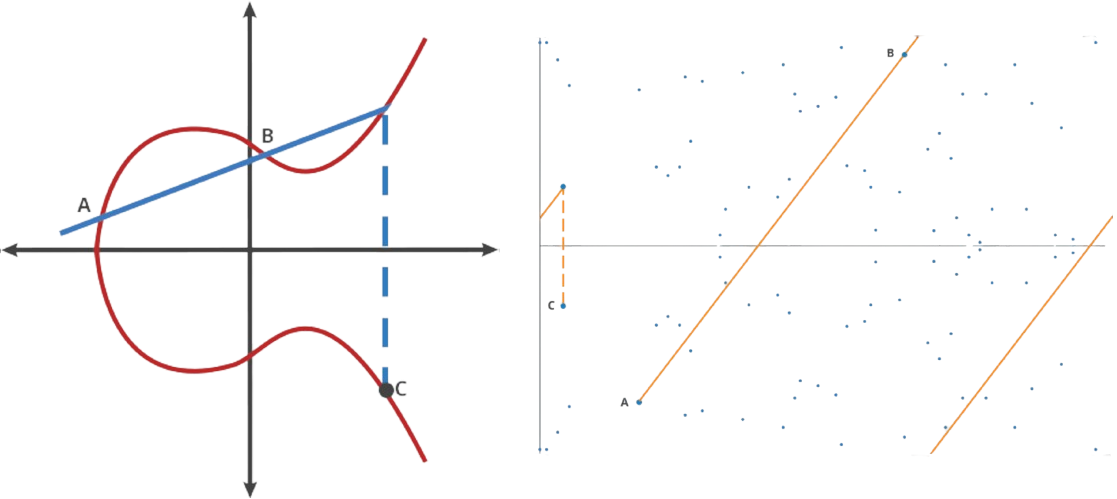
\includegraphics[width=1\linewidth]{resources/img/elliptic_curve.png}
		\caption{Two visual representations of an elliptic curve (from \url{https://blog.cloudflare.com/a-relatively-easy-to-understand-primer-on-elliptic-curve-cryptography/}). On the left, the cubic equation drawn as a curve on a Cartesian graph. On the right, the set of solutions $(x, y)$ to the cubic equation. Each representation also comprises a point addition operation between two points $A$ and $B$ resulting in a third point $C$}
		\label{figure:elliptic_curve}
	\end{center}
\end{figure}

Remarkably, $E(K)$ --- intended as the set of points of the elliptic curve --- is an abelian group, with the point at infinity $\mathcal{O}$ as the identity element and point addition ``$+$'' as the operation of the group. However, the addition of two points $P = (x_1, y_1)$ and $Q = (x_2, y_2)$ of an elliptic curve is not trivially equal to $(x_1+x_2, y_1+y_2)$. Instead, the addition of two points $P$ and $Q$ is defined as follows (see also \Cref{figure:elliptic_curve}):

\begin{itemize}
	\item draw the line connecting $P$ and $Q$ (if $P = Q$, then consider the tangent line as the line connecting $P$ and $Q$). The line will intersect the cubic equation in a third point denoted with $-R$ (if the line is vertical, use the point at infinity $\mathcal{O}$ as the result of $P + Q$\footnote{In fact, if the line is vertical, $P = -Q$, hence $P + Q = P - P = \mathcal{O}$ (in elliptic curves, the negative of a point $P(x, y)$ is defined as the point with the same $x$ but the negative $y$, i.e., $-P(x, -y)$). From this we also get that the point at infinity $\mathcal{O}$ is the identify element for the point addition operation, as $P - P = \mathcal{O}$ implies that $P + \mathcal{O} = P$});
	\item reflect $-R$ across the x-axis to get a new point $R$ which is defined to be $P + Q$;
	\remarkBlock{Actual formula to calculate the coordinates of $R$}{If $P \neq Q$ and $P, Q \neq \mathcal{O}$, given $(x_P, y_P)$ the coordinates of $P$ and $(x_Q, y_Q)$ the coordinates of $Q$, then the coordinates($x_R, y_R$) of $R$ are computed as $x_R = s^2 - x_P - x_Q$ and $y_R = -y_P + s \cdot (x_P - x_R)$, where $s = (y_P - y_Q) / (x_P - x_Q)$}
\end{itemize}

The point addition operation between $P$ and $Q$ when $P = Q$ --- that is, summing a point to itself --- is called \textbf{point doubling} and is denoted with $2P$. Generalizing, $nP$ denotes adding the point $P$ to itself $n$ times. Notably, given two integers $n$ and $m$, $m(nP) = n(mP)$ --- because the point addition operation is associative.

\readBlock{More information on elliptic curves}{The Cloudflare's blog post ``A (Relatively Easy To Understand) Primer on Elliptic Curve Cryptography'' --- available at the link \url{https://blog.cloudflare.com/a-relatively-easy-to-understand-primer-on-elliptic-curve-cryptography/} --- is an excellent source of more information on elliptic curves.}

\remarkBlock{Different ways to write down elliptic curve equations}{The cubic equation $y^2 = x^3 + ax + b$ is also called \textbf{Weierstrass form} or \textit{Weierstrass equation}. However, note that elliptic curves may be represented in other forms as well, such as the \textbf{twisted Edwards form} ($ax^2 + y^2 = 1 + dx^{2}y^{2}$, with $a,d \neq 0$) and the \textbf{Montgomery form} ($By^2 = x^3 + Ax^2 + x$).}

\paragraph*{Popular Elliptic Curves.} Intuitively, not all elliptic curves are suitable for cryptographic use; a random curve is most likely insecure in that sense. Therefore, elliptic curves are usually chosen from a list of standard options carefully curated by mathematicians and cryptographers. The most common elliptic curves are:

\begin{itemize}
	\item \textbf{P-256} --- also known as NIST P-256, secp256r1 or prime256v1: defined in Weierstrass form over the finite prime field $\mathbb{F}\textsubscript{p}$ with modulus $p = 2^{256} - 2^{224} + 2^{192} + 2^{96} - 1$. This curve is commonly used in \gls{tls} (\Cref{sec:popular_protocols:tls});
	\warningBlock{Beware of P-256}{P-256 was created by the \gls{nist} with supposedly random coefficients. However, since this claim is not verifiable, some mathematicians and cryptographers suspect the \gls{nsa} to have added a backdoor to this curve (see, e.g., \url{https://words.filippo.io/dispatches/seeds-bounty/}).}
	\item \textbf{secp256k1}: defined in Weierstrass form over the finite prime field $\mathbb{F}\textsubscript{p}$ with modulus $p = 2^{256} - 2^{32} - 977$. This curve is used in blockchains for cryptocurrencies like Bitcoin and Ethereum (\Cref{sec:popular_applications:blockchain});
	\item \textbf{Curve25519}: defined in Montgomery form over the finite prime field $\mathbb{F}\textsubscript{p}$ with modulus $p = 2^{256} - 19$. This curve is widely used for \gls{dh} key establishment (\Cref{sec:diffie_hellman}) in many modern protocols such as \gls{tls}, Signal, and WireGuard (\Cref{sec:popular_cryptographic_protocols}). The \gls{dh} key establishment over Curve25519 is called \textbf{X25519}. Also, Curve25519 is free from known patents and is recommended by \gls{nist} \cite{chen_recommendations_2023} and in RFC 7748 \cite{rfc7748};
	\item \textbf{Ed25519}: defined in twisted Edwards form over the finite prime field $\mathbb{F}\textsubscript{p}$ with modulus $p = 2^{256} - 19$. This curve is the bi-rational equivalent twisted Edwards form of Curve25519 (the twisted Edwards form is optimized for operating with digital signatures --- see \Cref{sec:digital_signatures});
	\item \textbf{Ed448} --- also known as Ed448-Goldilocks: defined in twisted Edwards form over the finite prime field $\mathbb{F}\textsubscript{p}$ with modulus $p = 2^{448} - 2^{224} - 1$. This curve is a larger variant of Ed25519;
	\item \textbf{BLS12-381}: defined in (short) Weierstrass form over the finite prime field $\mathbb{F}\textsubscript{p}$ with modulus $p$ being a 381-bit prime number. This curve is used for \gls{bls} signatures (\Cref{sec:digital_signatures:ciphers}) and blockchain applications (\Cref{sec:popular_applications:blockchain}) --- in fact, BLS12-381 is a pairing-friendly curve (\Cref{sec:trapdoor_functions:elliptic_curve_cryptography:pairings}).
	\curiosityBlock{What do numbers in the names of elliptic curves mean?}{Numbers in the name of elliptic curves typically refer to the underlying modulus. For instance, the curves P-256 and secp256k1 have ``256'' in their name due to the modulus of their finite prime field (which defines the order of the finite prime field, hence the number of elements in the finite prime field). Similarly, the curves Curve25519 and Ed25519 have ``25519'' as the underlying modulus is $p = 2^{256} - 19$. Curves with the same (literal part of the) name but different numbers typically denote different sizes of the same curve. For instance, P-256, P-384 (also known as secp384r1), and P-521 (also known as secp521r1) denote the same curve over different moduli; as a rule of thumb, bigger curves offer more cryptographic security at the expense of (computational and space) efficiency.}
\end{itemize}

The choice of the elliptic curve and its form greatly influence the security and efficiency of algorithms.

\readBlock{More information on the choice of elliptic curves}{Bernstein's and Lange's blog post ``SafeCurves: choosing safe curves for elliptic-curve cryptography'' --- available at the link \url{https://safecurves.cr.yp.to/} --- is an excellent source of more information on how to choose elliptic curves (and how their secure implementation is often harder than it seems).}
